%% Schematic of the stage crossover: the 2x2 design that separates direct from inherited
%% dependence, and the per-stage verdicts it produces on one scenario.
%% Artwork regenerated by scripts/make_fig_scaff.py. The `paper' variant is used here because it
%% is drawn 1:1 at ACM text width; v1--v4 carry the same content at presentation size and are
%% drop-in replacements only where the figure is reproduced large (slides, poster).
\begin{figure*}[t]
  \centering
  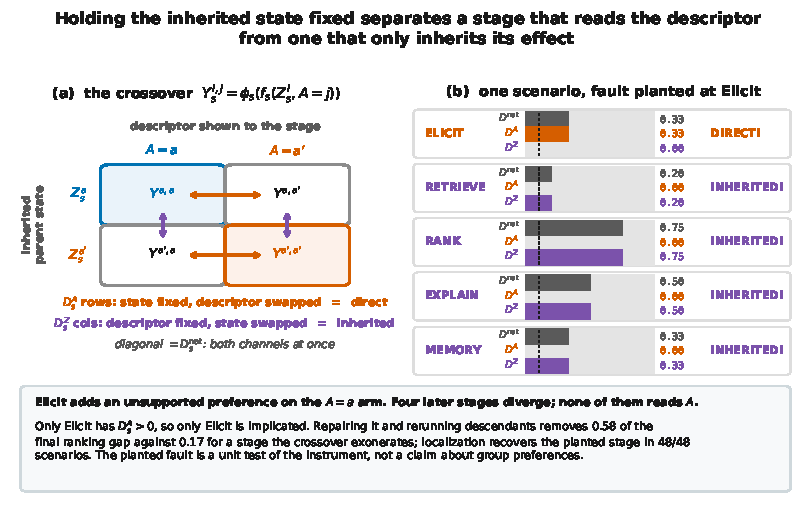
\includegraphics[width=\linewidth]{figures/fig_scaff_paper.pdf}
  \caption{The stage crossover. (a) Each stage is re-run four times: the row index selects whose
    inherited parent state $Z_s$ the stage is supplied, the column index selects which descriptor
    the stage itself is shown. Contrasting along a row holds the state fixed and isolates the
    stage's own response, $D^{A}_s$; contrasting down a column holds the descriptor fixed and
    isolates what the stage inherited, $D^{Z}_s$. The diagonal is natural divergence
    $D^{\mathrm{nat}}_s$, which confounds the two. (b) One scenario in which \stage{Elicit} adds
    a preference the latent profile does not support. Four later stages diverge, so
    $D^{\mathrm{nat}}_s$ implicates all of them; only \stage{Elicit} has $D^{A}_s > 0$, and every
    later stage's divergence is carried entirely by $D^{Z}_s$. The dashed line is the decision
    margin. Values are the primary per-stage coordinate of the controlled prototype
    (Section~\ref{sec:scaff-results}); the planted fault is a unit test of the instrument, not a
    claim about group preferences.}
  \Description{A two-panel schematic. The left panel is a two-by-two grid of crossover outcomes,
    with rows labelled by which arm's inherited parent state is supplied and columns by which
    protected descriptor the stage is shown; horizontal arrows between cells are labelled direct
    sensitivity and vertical arrows are labelled inherited dependence. The right panel lists the
    five pipeline stages, each with three horizontal bars for natural, direct and inherited
    divergence and a verdict label: DIRECT for Elicit and INHERITED for Retrieve, Rank, Explain
    and Memory.}
  \label{fig:scaff}
\end{figure*}
